\documentclass[10pt,a4paper]{article}
\usepackage{amsmath}
\usepackage[utf8]{vietnam}
\usepackage{amsfonts}
\usepackage{amssymb}
\usepackage{graphicx}
\usepackage[left=2cm,right=2cm,top=2cm,bottom=2cm]{geometry}
\setlength{\parindent}{0pt}
\begin{document}

\begin{center}
    \fontsize{30}{30}\selectfont
    CƠ SỞ TOÁN HỌC
\end{center}
\fontsize{14}{20}\selectfont
Gồm 2 bước:\\
- Bước 1: Tính độ phức tạp để thực hiện tính F[i, j] cho mọi j ở mỗi node i.\\
- Bước 2: Tính tổng độ phức tạp của các node.\\
\section[\textbf]{Bước 1}
Giả sử node i có $p_i$ node con.\\
Kích thước (tổng số node con + 1) khi khởi tạo là sz[i]=1.\\
Độ phức tạp để tính F[i, j] trong node i khi nhập cây con thứ nhất vào i là\\
sz[i] * sz[1] = 1 * sz[1]\\
Sau đó cập nhật sz[i] += sz[1] -> sz[i]=1+sz[1]\\
Độ phức tạp để tính F[i, j] khi thêm cây con thứ hai vào i là \\
sz[i]*sz[2]=(1+sz[1])*sz[2]\\
Cập nhật sz[i]= 1 + sz[1] + sz[2]\\
Độ phức tạp để tính F[i, j] khi thêm cây con thứ ba vào i là\\
(1+sz[1]+sz[2]) * sz[3]\\
...\\
Độ phức tạp để tính F[i, j] khi thêm cây con cuối vào i là\\
(1+sz[1]+...+sz[$p_i$-1])*sz[$p_i$]\\
\fontsize{14}{25}\selectfont
Vậy độ phức tạp để tính F[i, j] của node i sau khi cập nhật hết cây con là\\
1*sz[1]+ (1+sz[1])*sz[2] + (1+sz[1]+sz[2])*sz[3] + ... + (1+sz[1]+...+sz[$p_i$-1])*sz[$p_i$]\\
= $\sum_{u=1}^{p_i}(sz[u])$ + $\sum_{u=1, v=u+1}^{p_i}(sz[u]*sz[v])$\\
= $\sum_{u=1}^{p_i}(sz[u])$ + $\sum_{u \neq v}^{}(sz[u]*sz[v])$\\
Ta có O($\sum_{u=1}^{p_i}(sz[u])$ + $\sum_{u=1, v=u+1}^{p_i}(sz[u]*sz[v])$)\\
= O(max($\sum_{u=1}^{p_i}(sz[u])$ , $\sum_{u=1, v=u+1}^{p_i}(sz[u]*sz[v])$))\\
= O($\sum_{u=1, v=u+1}^{p_i}(sz[u]*sz[v])$)\\
Vậy độ phức tạp để tính F[i,j] cho node i là\\
O($\sum_{u=1, v=u+1}^{p_i}(sz[u]*sz[v])$)\\
hay O($\sum_{u \neq v}^{}(sz[u]*sz[v])$)\\
Lại có $\sum_{u \neq v}^{}(sz[u]*sz[v])$ = $\dfrac{2(\sum_{u \neq v}^{}(sz[u]*sz[v]))+\sum_{u=1}^{p_i}(sz[u])^2-\sum_{u=1}^{p_i}(sz[u])^2)}{2}$\\
=$\dfrac{1}{2}$*$((\sum_{u=1}^{p_i}sz[u])^2-\sum_{u=1}^{p_i}(sz[u])^2)$ (1)\\
mà sz[i]= $\sum_{u=1}^{p_i}sz[u]$\\
(1) <=> $\dfrac{1}{2} * ((sz[i])^2-\sum_{u=1}^{p_i}(sz[u])^2)$\\
=> Độ phức tạp để tính F[i, j] ở mỗi node i là O($(sz[i])^2-\sum_{u=1}^{p_i}(sz[u])^2$)\\

\fontsize{14}{25}\selectfont
\section[\textbf]{Bước 2}
Độ phức tạp ở mỗi node v là O($(sz[v])^2-\sum_{i=1}^{p_v}(sz[i])^2$)\\
Độ phức tạp của node lá z là O($(sz[z]^2)-0$)=O($(sz[z])^2$)\\
Độ phức tạp của bài toán có n node: $\sum_{k=1}^{n}O((sz[k])^2-\sum_{l=1}^{p_k}(sz[l])^2)$\\
=O($sz[1]^2$) = O($n^2$) do sz[1]=n hay cây bắt đầu từ node root 1 có kích thước là n\\
\bfseries 
Ví dụ minh họa
\mdseries
\begin{center}
     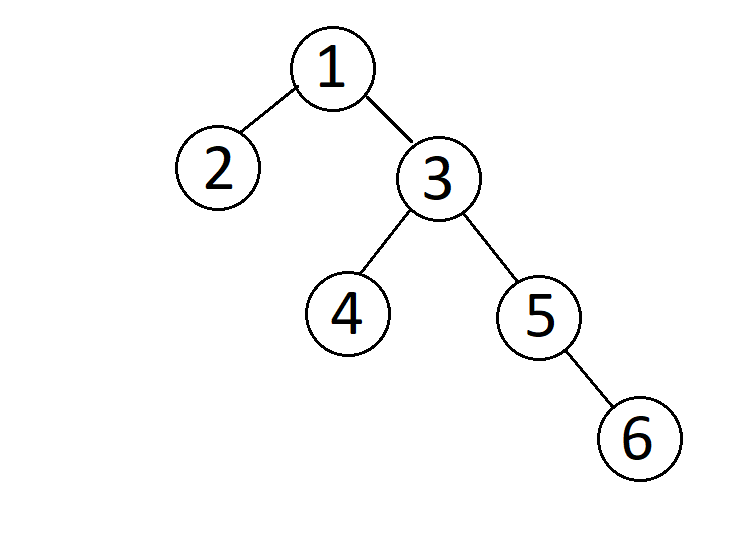
\includegraphics[scale=.5]{vidu.png} \\
\end{center}

\begin{flushleft}
Độ phức tạp để tính F[i, j] ở node 2: $(sz[2])^2$\\
Tương tự: \hspace{3.7 cm}node 4: $(sz[4])^2$\\
\hspace{6 cm}node 6: $(sz[6])^2$\\
Độ phức tạp để tính F[i, j] ở node 5: $(sz[5])^2-(sz[6])^2$\\
Tương tự: \hspace{3.7 cm}node 3: $(sz[3])^2-(sz[4])^2-(sz[5])^2$\\
\hspace{6 cm}node 1: $(sz[1])^2-(sz[2])^2-(sz[3])^2$\\
\end{flushleft}

Độ phức tạp của bài toán: $(sz[1])^2+(sz[2])^2-(sz[2])^2+(sz[3])^2-(sz[3])^2+(sz[4])^2-(sz[4])^2+(sz[5])^2-(sz[5])^2+(sz[6])^2-(sz[6])^2$=$(sz[1])^2$=$6^2$
\end{document}